\renewcommand{\chaptername}{Programación sobre plataforma Arduino UNO}

\chapter{Programación sobre plataforma Arduino UNO} \label{ap:ard_uno_env}
%\markright{Programación sobre plataforma Arduino Uno}
\section{PlatformIO }

En este trabajo, no se utiliza el IDE provisto por la plataforma de Arduino, sino, que se utiliza PlatformIO. Para instalar platformIO, debe instalarse el editor de código VisualStudioCode. Este es gratuito, multiplataforma, y se encuentra disponible en \url{https://code.visualstudio.com/}. 

Una vez instalado el editor de código, se debe instalar el plugin de PlatformIO, el cual es una extensión de Visual Studio Code, que permite programar sobre casi cualquier sistema embebido. Para instalar este plugin, dentro del editor de código, debe realizar un clic en el cuadrado rojo, que se muestra la siguiente imagen: 

\begin{figure}[ht!]
	\hspace{-20mm}
	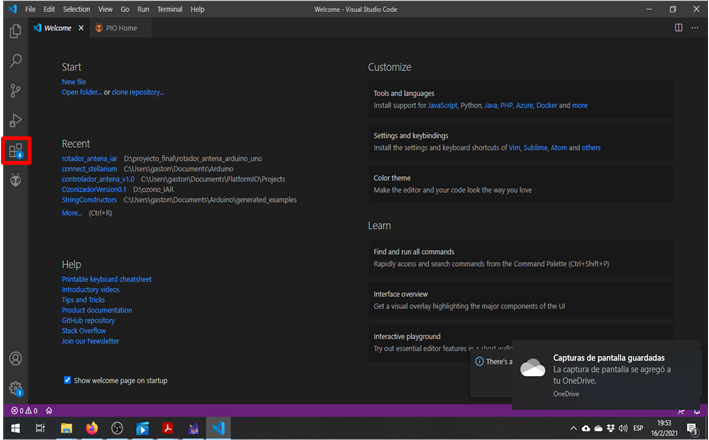
\includegraphics{Apéndice/ard_uno/platformIO}
	\caption{imagen de Visual Studio Code para añadir extensiones}
	\label{ref:platformIO}
\end{figure} 

Luego, se abre una ventana donde puede introducir texto, en esta debe introducir ``PlatformIO'', y en la parte derecha de la misma, le aparece, el botón de instalar en azul. Una vez se realicen estos pasos, se puede iniciar un nuevo proyecto dentro de este pluggin. La explicación del inicio de un nuevo proyecto, y el proceso de instalación detallado, rebasa el alcance del presente informe. 


\section{Configuración de platformIO}

Una vez, iniciado un nuevo proyecto en platformIO, aparecen, las siguientes carpetas y archivos en el directorio principal del proyecto:
 
\begin{itemize}
	\item carpetas: 
	\begin{itemize}
		\item .pio 
		\item .vscode 
		\item include 
		\item lib 
		\item src 
		\item test 	
	\end{itemize}
	\item archivos: 
	\begin{itemize}
		\item .gitignore 
		\item platformio.ini  
	\end{itemize}
\end{itemize}

Las carpetas .pio y .vscode, tienen configuraciones relacionadas al proyecto(compilador, librerías, ruta del compilador, etc). El archivo .gitignore, está relacionado con el sistema de control de versiones git, en este trabajo, se utilizó este sistema de control de versiones. La explicación del mismo, rebasa el alcance de este texto. El otro archivo, se relaciona con la configuración de platformIO. Este, se modifica, para que se pueda realizar la compilación. 

Dentro de estas carpetas, las que se utilizan en el proyecto, son las carpetas include, lib y src. 

La carpeta include, contiene todos los archivos de cabecera que utiliza el proyecto, estos, en general tienen extensión .h. La carpeta lib, incluyen las librerías, tanto las desarrolladas por terceros, como las que se desarrollen en el proyecto, y la carpeta src, contiene el archivo principal del programa. 

En el programa desarrollado en el presente texto, dentro de la carpeta include, se crean dos carpetas, denominadas ``lectura\_encoders'' y ``control\_motores''. Dentro de estas carpetas, se colocan los archivos ``lectura\_encoders.cpp'',  ``lectura\_encoders.h'',  ``control\_motores.h'' y ``control\_motores.cpp''(ver anexo del capítulo \ref{app:capsoft} y código versión final). 

Una vez, creados estos archivos, dentro de la carpeta lib, se crea una nueva carpeta, denominada ``tiempo'', donde se guardan los archivos ``tiempo.cpp'' y ``tiempo.h''. 

Una vez, finalizada la creación de archivos y carpetas, se debe proceder a configurar el entorno de desarrollo. El entorno de desarrollo, se configura, mediante el archivo platformio.ini. 

La programación del archivo platformio.ino, puede encontrarse en \cite{platformio}. En, esta referencia, se explica que un proyecto, puede poseer distintos entornos. En el caso del presente trabajo, se utiliza un solo entorno. La sentencia para crear el entorno es \mintinline{ini}{[env:entorno]}, donde entorno, se le debe dar el nombre que el programador desee.  

Luego de este paso, se debe configurar, la búsqueda de los archivos dentro de los directorios. Esto, según el propio compilador, debe tener la directiva ``-I''. Esta directiva se da dentro del archivo platformio.ini, con la sentencia \mintinline{ini}{build_flags}. Esta, permite, adicionar todas las banderas de compilación, que se deseen, donde deben separarse por comas o por saltos de líneas. En este trabajo, se opta por la segunda. Estas, son algunas de las modificaciones del archivo platformIO.ini. El resto de las modificaciones, están relacionadas con el directorio de trabajo, y con avisos relacionados al compilador. El archivo platformio.ini resulta finalmente de la siguiente manera: 

\begin{listing}[ht!]
	\begin{minted}[frame=single,linenos,breaklines]{ini}
		
[env:uno]
platform = atmelavr
board = uno
framework = arduino
lib_extra_dirs=D:\proyecto_final\rotador_antena_arduino_uno\rotador_antena_iar\include\
build_flags = -Wchar-subscripts
   -Wunused-variable 
   -DCORE_DEBUG_LEVEL=5 
   -I\include\control_motores
   -I\include\lecturas_encoders		
lib_deps = 
		paulstoffregen/Ethernet@0.0.0-alpha+sha.9f41e8231b
		marcoschwartz/LiquidCrystal_I2C@^1.1.4
	\end{minted}
\caption{Modificaciones realizadas sobre el archivo platformio.ini}
\end{listing}

Todos estos archivos y modificaciones, se encuentran en el sistema de control de versiones con soporte para git: github. El enlace al proyecto es \url{https://github.com/gaston-cb/control_antena_iar}


\section{Carga de software dentro del microcontrolador} 

Una vez, se ha creado un proyecto, y se configura, el siguiente paso, es crear un primer programa, y cargarlo dentro del microcontrolador. Para esta sección, puede utilizar algún ejemplo que este incluido dentro del software platformio, o puede buscar algún ejemplo en Internet. Una vez realizado este proceso, se crea un nuevo proyecto, o se abre algún proyecto existente dentro de platformIO, y en la parte inferior izquierda de la pantalla, aparecen los iconos para compilar, cargar,etc. Estos iconos son los siguientes: 

\begin{itemize}  
%	\renewcommand{\labelitemi}{\raisebox{-3.2\height}{\huge}}
    \item[]\hspace{-20mm}
\includegraphics{Apéndice/ard_uno/icon_1} Marca errores de sintaxis y de compilación. 	
    \item[] \hspace{-10mm} 
\includegraphics{Apéndice/ard_uno/icon_2} Acceso al menú principal de platformIO. 
	\item[] \hspace{-10mm} 
\includegraphics{Apéndice/ard_uno/icon_3} compilar. Genera los archivos binarios. Puede cambiarse el directorio de compilación mediante el archivo platformIO.    
	\item[] \hspace{-10mm} 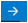
\includegraphics{Apéndice/ard_uno/icon_4} Sube el archivo a la placa arduino. No requiere seleccionar el puerto. El programa analiza los puertos, y los sube automaticamente. 	
	\item[] \hspace{-10mm} 
\includegraphics{Apéndice/ard_uno/icon_5} Borra todos los archivos generados por la compilación. 
	\item[] \hspace{-10mm} 
\includegraphics{Apéndice/ard_uno/icon_6} Visualizar el puerto serie. 
\end{itemize}
 
Presionando el botón que tiene una flecha hacia la derecha, con el microcontrolador conectado a la PC, se carga el software de forma automática. 




\section{Compilación condicional}

La compilación condicional consiste en utilizar lo que se denomina directivas de compilación. El código es muy similar a lo que se realiza en programación, pero puede compilar diferentes códigos. Para realizar este tipo de compilación, deben definirse banderas o flags de compilación, y con una estructura similar al ``if - else'', puede seleccionar el código que se carga dentro del microcontrolador. Para ilustrar la compilación condicional, se utiliza el siguiente código 
\begin{listing}[ht!]
	\begin{minted}[linenos,frame=single,texcomments]{Arduino}
#define BANDERA 5 

void setup()
{
#if BANDERA<5
	Serial.begin(9600) ; 
#else
	 Serial.begin(115200) ; 		
#endif
... 
}

void loop()
{
 ... 
}
	\end{minted}
\caption{Código ejemplo para ilustrar la compilación condicional.}
\label{cod:ejemplo_comp_cond}
\end{listing}
 
En el código anterior, se define la bandera, con el nombre \mintinline{Arduino}{BANDERA}, y se le asigna el valor de 5.  

Luego dentro de la función setup, se encuentran las sentencias de las líneas 5 a 9. En el código de ejemplo, cambia el baudrate del puerto UART del microcontrolador. En este ejemplo, el baudrate seleccionado es de 115200bps(bits por segundo). Si por el contrario, por ejemplo, se pone la variable BANDERA en 2, el baudrate seleccionado sería el de 9600bps. Esto, puede usarse por ejemplo, para trabajar con dos arquitecturas diferentes, con el mismo código y que trabajen bajo el entorno Arduino.     
 
La compilación condicional, pueden anidarse tantos ``if-elsif-else'' cómo se deseen, y puede ser tan complejo como un lenguaje de programación propio. En este documento, la única sentencia que se ha usado de las directivas de compilación es esta, y es la única que se muestra.   




\section{Sentencias sobre el entorno arduino}

El código Arduino, provee de sus funciones, las cuales permiten el manejo del hardware con una mayor flexibilidad, sin entrar en el detalle del conocimiento profundo del hardware. Algunas de las sentencias provistas por su lenguaje propio son: 
\begin{itemize}
	\item \mintinline{Arduino}{analogRead(PORTPIN)}: devuelve el valor del puerto analógico digital. En PORTPIN, debe ingresar el valor del puerto analógico que se desea leer. 
	\item \mintinline{Arduino}{pinMode(NUMBER\_PIN,MODE)}: permite poner el puerto en tres modos distintos, estos son: 
		\begin{itemize}
			\item INPUT: pone el pin como entrada
 			\item INPUT\_PULLUP: pone el pin como entrada, pero pone una resistencia de pull-up desconocida. Según \cite{ATmega328P} esta oscila entre 20K$\Omega$ y 50K$\Omega$ 
			\item OUTPUT: permite poner el puerto como salida. 
		\end{itemize}
	\item \mintinline{Arduino}{digitalRead(PORTPIN)} y \mintinline{Arduino}{digitalWrite(PORTPIN,STATE)}: En el caso de digitalRead, lee el puerto de entrada, y devuelve el estado de este. En el caso de digitalWrite, escribe el puerto definido como salida, STATE, puede ser LOW o HIGH.   
\end{itemize}

Estas son solo algunas de las funciones que provee el entorno Arduino para el manejo de puertos del microcontrolador. Para una lista completa, la puede obtener de \url{https://www.arduino.cc/reference/en/}

\section{Conversor Analógico Digital}

En el mundo real, las señales electricas, son analógicas. Estas, se pueden digitalizar, para poder procesarlas dentro de un microcontrolador,pc ,etc. Este transpaso de señales eléctricas analógicas a digitales, las realiza un componente de hardware, que se denomina conversor analógico-digital. Este dispositivo, convierte un nivel de tensión eléctrica en un número binario. La cantidad de bits que tenga este número binario, define la resolución del conversor. Además, en caso de trabajos futuros, debe considerarse el error introducido por el mismo, ya que el último bit en general es incierto (esto se denomina 1/2LSB en las hojas de datos generalmente). 

En el caso del microcontrolador Arduino UNO, este posee integrado un conversor analógico-digital, lineal, de 10 bits de resolución. Al ser 10 bits, la cantidad de niveles que puede tomar es de $2^10 = 1024$, o sea que va desde 0 a 1023. La tensión de este, va desde 0 a 5volts. Para calcular cual es el mínimo valor de tensión, que hace que se incremente en un bit viene dado por: 
\[
	\frac{5V}{1024} = 0.0048V 
\] 
O sea, que el conversor posee una resolución de aproximadamente 0.5mv. 

Para leer el conversor analógico digital, debe usarse la función analogRead(PORTPIN), y luego almacenar ese valor en una variable. Este valor, estará, entre 0 y 1023. El código para leer el conversor analógico digital, por ejemplo, del puerto A0, es el siguiente: 
\begin{minted}[linenos,frame=single,escapeinside=||]{Arduino}
#define PORT_PIN A0 

| Leer puerto analógico A0  |

int lect_ad = analogRead(PORT_PIN) ; 


\end{minted} 
